\chapter{時間軸セグメントを導入したHTM}
\section{提案モデルの概要}
従来のHTMは1つ前の時刻におけるパターンを表現するセルのみとの接続を持つように学習していたが、前章で述べたように長期依存考慮に関して性能が低いという問題があった。
そこで、その問題を解消するために接続セグメントに時間軸を導入することによって、複数前の時刻におけるパターンを表現するセルとの接続も持つように学習させた。

この改良の重要な点は新たに接続をもつようになった時刻の範囲においてのみに長期依存関係を保持できるようになったということではない。
HTMの学習において予測状態に遷移するセルに関して適切な密度を保持し続けることは重要な要素である。
改良したHTMは複数前の時刻にわたって接続を学習することによって、適切な密度が保持されセルの状態遷移が安定して行われる。
それによって新たに接続を持つようになった時刻の範囲をはるかに超える長期依存考慮が可能になった。

前章で挙げた以下の2つの問題点に関して、この改良の効果を具体的に述べる。

\begin{enumerate}
  \item 疎な分散表現を用いたために発火するセルが徐々に少なくなり消失する。
  \item 学習が大きく進んだパターンにおいて表現が疎になった時に次のパターンに繋がっていたセルが消失するために学習状態が損失する。
\end{enumerate}

まず1の問題に関しては複数前の時刻における活性化状態とそれらのセルとの接続セグメントを用いて予測状態のセルの計算を行い、それによるすべての予測状態のセルを予測に用いるためにセルの減少が抑制されている。

次に2の問題に関しては学習が大きく進んだパターンにおいて表現が疎になった場合でも複数の時刻にわたる接続があることによって学習状態の損失が抑制されている。
これは次のパターンの予測に用いる学習が複数の時刻間に分散されているためである。

以上の2つの問題点の抑制によって長期依存考慮に関する性能が向上した。

\section{提案モデルの構造}
\subsection{従来型と同じ部分}

HTM全体の構造やセルの状態遷移、パターンの表現は従来のHTMを用いた。

\subsection{セル内の構造}

\begin{figure}[ht]
  \begin{center}
    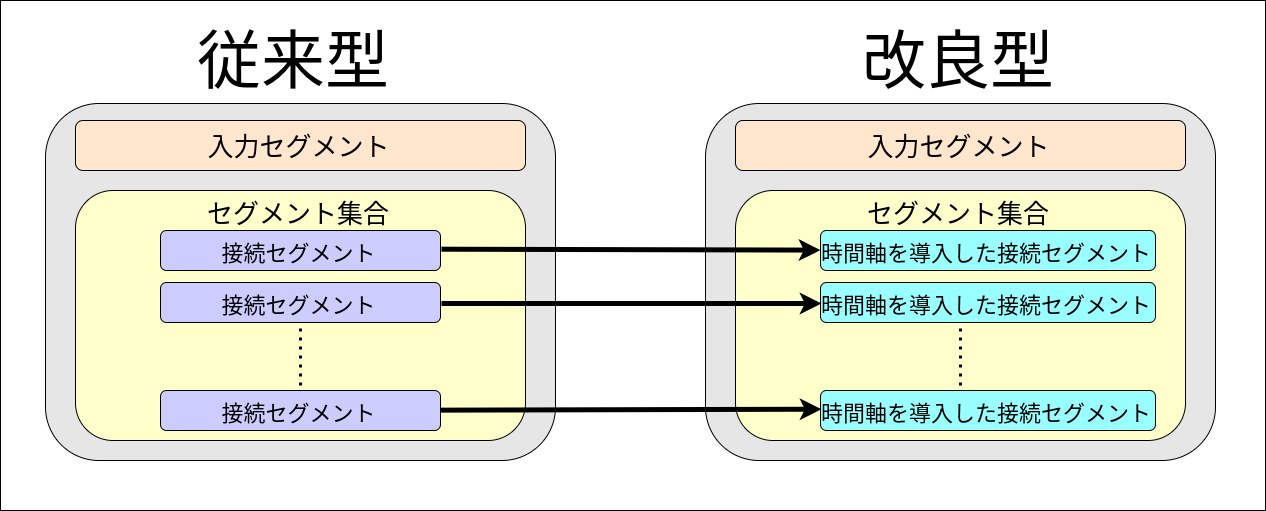
\includegraphics[width=14cm]{./fig/drawing_9}
    \caption{提案モデルにおけるセル内の構造}
    \label{fig:HTM_improved}
  \end{center}
\end{figure}

提案モデルのセル内の構造は図3.1のようになっている。
入力セグメントは従来型のHTMと同様になっているが、セグメント集合の構造は異なっている。
セグメント集合内の接続セグメントに関して時間軸を導入した。
これによって接続セグメントはHTM中のすべてのセルとの接続値と時間軸の3次元テンソル値によって表される。
そのためセグメント集合は4次元のテンソル値となる。

\section{提案モデルの学習アルゴリズム}
提案モデルは従来のHTMを拡張しているため学習アルゴリズムにおいても拡張する必要がある。
時間軸を導入したことによって予測状態のセル計算とセグメント集合を用いた接続値の更新において変更を加えた。

\subsubsection{従来型と同じ部分}

活性化状態のセルの計算に関しては従来のHTMと同様である。

\subsection{予測状態のセルの計算}
時間軸セグメントの長さを$\tau_c$とし、セグメント集合における接続値を${\bf D}^d_{ij}(\tau)$とする。
また接続値がしきい値を超えた値のみを取り出し、接続の可否のみを表した2進行列を${\bf \tilde{D}}^d_{ij}(\tau)$とする。

\begin{equation}
  \pi^t_{ij} =
  \left\{
  \begin{alignedat}{2}
    1 \qquad &if \; \exists_\tau \exists_d\|{\bf \tilde{D}}^d_{ij}(\tau) \circ {\bf A^t}\|_1 > \theta \quad (t-\tau_c < \tau < t-1)\\
    0 \qquad &otherwise
  \end{alignedat}
  \right.
\end{equation}

\subsection{セグメント集合を用いた接続値の更新}
セグメントを更新する場合分けは従来型と同様となっている。
またセグメントの更新式も従来型と同様となっており式2.6と式2.7となっているが、セグメントの更新を複数の時間($t-\tau_c < t-1$)にわたって適用するように変更している。
